\subsubsection{About}

Decision trees are one of the older concepts of predicting \parencite{friedl1997decision}. The idea is to determine if something goes on the left or right path. Example image bellow shows how decisions are made with it.
\begin{figure}[H]
    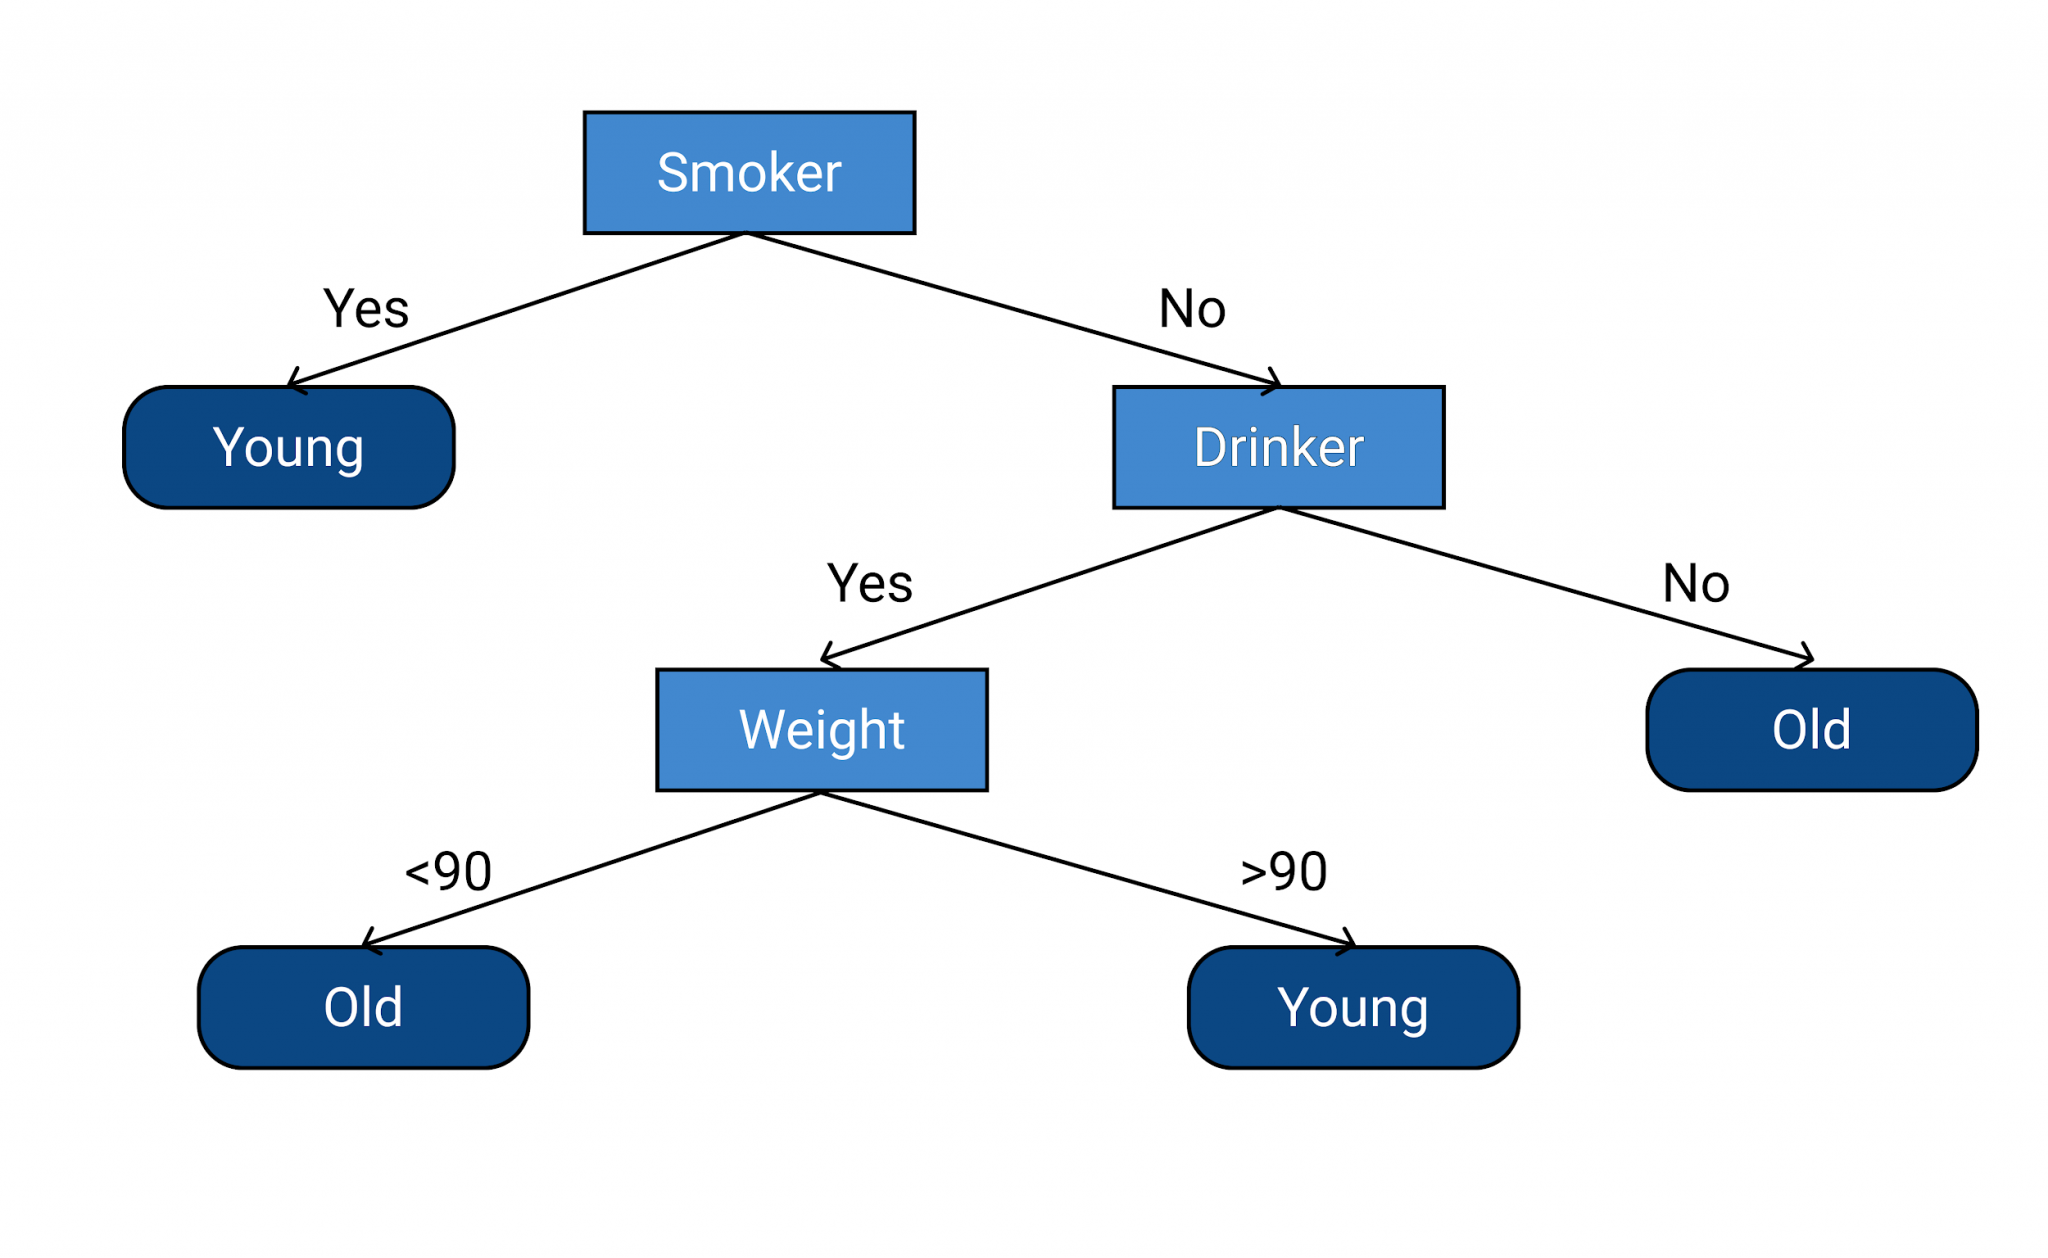
\includegraphics[scale=0.20]{img/Classification/dtree.png}
    \centering
    \caption{Decision tree showcase \parencite{web:Upgrad}}
    \label{fig:Dtree}
\end{figure}

In our case we have used MLlib library from PySpark in order to use one of preexisting models.